\section{Empirical Results}
\label{sec:results}

\subsection{Univariate Models}

The results for the univariate model fit are presented in table
\ref{table:MAEunivariate}.  For all of the univariate models described
in section \ref{sub:univariate} a Wald test assessing the empirical
evidence for a restricted structural model is computed. I find that
the joint Null of the Frenkel-Bilson model cannot be rejected on a 1\%
confidence level for the simple OLS modeling of FX-rates.  We
proceeded therefore to estimate the out of sample performance for the
OLS applying both the most general structural model and the
Frenkel-Bilson model.

For the transfer function model described in \ref{eq:transfer} the
rate of decay, the persistence term and the dead lag were estimated at
each model estimation in the rolling forecast. The optimal lags for
the terms above where selected minimizing the Akaike information
criteria (See Akaike (1998, \cite{Akaike}). I found a compelling
evidence for modeling the differentiated series with one term in the
nominator capturing the effect of unexpected shifts in the independent
variables and two terms in the denominator capturing the general high
persistence of FX-rates movements through time.

The results of table \ref{table:MAEunivariate} confirm the one of the
general literature where an OLS model vastly under-performs a random
walk in the out of sample forecast of FX-rate at all tested lags.

\begin{table}[!ht] % ! -> to insert at the bottom of a page.
  \centering
  \caption[MAE \textendash \ Univariate Models]{Mean Absolute Error \textendash \ Univariate Models
           Equal Predictive Ability p-value in Parenthesis}
  \begin{tabular}{llccc} % tells how you want the columns aligned.
    \toprule
    \multicolumn{5}{c}{Univariate Models}                      \\
    \cmidrule(r){1-5}
    Lag                           &   Model                                     &Switzerland  & United Kingdom  & Japan\\
    \midrule
    \multirow{4}{*}{MAE 1}        & \multicolumn{1}{l}{Random Walk}             &   0.0193 (0.503) & 0.0168 (0.506) & 0.0162 (0.506)\\
                                  & \multicolumn{1}{l}{Transfer Function Model} &   0.0205 (0.119) & 0.0176 (0.128) & 0.0173 (0.228)\\ 
                                  & \multicolumn{1}{l}{OLS - unrestricted}      &   0.0234 (0.031) & 0.0211 (0.053) & 0.0194 (0.192)\\
    \\
    \multirow{4}{*}{MAE 3}        & \multicolumn{1}{l}{Random Walk}             &   0.0390 (0.307) & 0.0330 (0.093) & 0.0291 (0.534)\\ 
                                  & \multicolumn{1}{l}{Transfer Function Model} &   0.0384 (0.499) & 0.0341 (0.094) & 0.0280 (0.111)\\
                                  & \multicolumn{1}{l}{OLS - unrestricted}      &   0.0603 (0.133) & 0.0443 (0.143) & 0.0497 (0.000)\\
    \\
    \multirow{4}{*}{MAE 6}        & \multicolumn{1}{l}{Random Walk}             &   0.0580 (0.483) & 0.0495 (0.785) & 0.0439 (0.484)\\
                                  & \multicolumn{1}{l}{Transfer Function Model} &   0.0581 (0.468) & 0.0498 (0.526) & 0.0442 (0.396)\\
                                  & \multicolumn{1}{l}{OLS - unrestricted}      &   0.0789 (0.003) & 0.0531 (0.486) & 0.0669 (0.000)\\
     \\
    \multirow{4}{*}{MAE 12}       & \multicolumn{1}{l}{Random Walk}             &   0.0964 (0.171) & 0.0584 (0.726) & 0.0753 (0.505)\\
                                  & \multicolumn{1}{l}{Transfer Function Model} &   0.0954 (0.489) & 0.0598 (0.678) & 0.0752 (0.147)\\
                                  & \multicolumn{1}{l}{OLS - unrestricted}      &   0.1210 (0.000) & 0.0744 (0.523) & 0.1001 (0.000)\\
    \bottomrule
  \end{tabular}
  \label{table:MAEunivariate}
  \vspace{2em}
\end{table}

In contrast, transfer function models performed much better in
modeling FX-rates out of sample. While the model still under-performs a
random walk in forecasting the FX-rates of the countries of interest
at 1 month lag, the evidence at higher lags is rather mixed and it
seems the two models performs equally in forecasting FX-rates out of
sample. This is confirmed by the superior predictive test of Hansen
(2005, \cite{HansenSPA}) and the p-value reported in parenthesis in
table \ref{table:MAEunivariate} obtained by the bootstrap method of
Hansen (2011, \cite{HansenMCS}).  For all of the models the equal
predictability hypothesis of the unrestricted and restricted OLS model
is rejected with 5\% confidence.

Two possible causes for such observations might exist. While on one
hand the increased forecast performance at higher lags might be
explained by the different information set provided to the two models
as described in \ref{sub:forecast}, on the other hand, the fact might
be caused by an increasing importance of macroeconomic variables for
explaining the long run behaviour of FX-rates movements.

Finally, the Null of equal predictability of the random walk model and
the transfer function models in the superior predictability test could
not be rejected with 10\% confidence. This suggests the random walk
model as the best univariate model to fit FX-rates out of sample given
its parsimonious computation power combined with a restricted
information set compared to the transfer function model as discussed
in \ref{sub:forecast}.

I observe no systematic difference when looking at RMSE. The picture
of the latter looks similar to the results obtained looking at the MAE
at all lags and for all models. No particularly important outliers in
forecast errors seem to be of significant importance in the analysis.
The final word is given to the directional accuracy measure defined as
the average number of times the sign of the realized FX-rate
difference is matched by an equivalent sign in the FX-rate forecast
difference. The values for such statistics lie between 0.4-0.6 for all
the frequencies and there does not seem to be systematic differences
among the models. 

\subsection{Multivariate Models}

The evidence from the previous section together with the general
empirical literature suggests the presence of a unit root in the
FX-rates. This was further confirmed by augmented Dickey-Fuller tests
(Dickey and Fuller (1979, \cite{DickeyFuller})) applied to the
FX-rates and macroeconomics variables at the moment of detrending the
series. There a statistically significant presence of unit roots could
be found in the series in level.  Dickey-Fuller tests were estimated
once again after differentiating the series. All of the series but the
US-JP interest rates differential and the US-UK unemployment rate
differential proved to be stationary after such adjustment, which
supports an evidence for an integration order of 1 for most of the
series.

While in the previous section the FX-rate unit root was proved to be
best modeled by a simple random walk model this section further
expands the analysis by looking at the performance of multivariate
models. Those may capture and efficiently estimate the relation among
macroeconomics variables and FX-rates in the case of endogeneity among
the series.

While the reference paper of Meese and Rogoff (1983a and 1983b,
\cite{MeeseRogoffa, MeeseRogoffb}) attempted to use a multivariate
model through a vector auto-correlation model I will analyze the
extent of co-integration among the series using the results of the
previous analysis showing a higher order integration for the
macroeconomic and FX-rates series.

In order to do that I tested the hypothesis of co-integration for the
macroeconomics variables and the FX-rates taking into account the
trend displayed by the times series. The results of this analysis are
based on the trace statistic for the computed eigenvector discussed in
Johansen (1991, \cite{Johansen}). Running the Johansen co-integration
test I obtained the results presented in table
\ref{tab:Co-Integration}. All of the series display a profound evidence
for the presence of two co-integration vectors at 5\% percent
confidence level.

Given the five series of macroeconomic fundamentals it is possible
that the two co-integration relations might exist just among such
variables and that a long term relation between the macroeconomic
fundamentals and the FX-rate for the three different series does not
exists. In order to test such a hypothesis I decided to first run
Johansen tests verifying for co-integration between the FX-rate and the
single macroeconomic variables. I then iterated the process by
gradually adding macroeconomic variables until the estimation of a
model included all of the variables present in the structural model as
in \ref{eq:structural}. The results in this case confirm the
hypothesis of co-integration between FX-rates and the macroeconomic
variables.  For the period analyzed I found strong evidence for
co-integration among the FX-rate and macroeconomic fundamentals for the
UK-US series. In such a case the Null of no co-integration could be
rejected with 5\% confidence for the FX-M3, FX-CPI, FX-Current
Account, FX-interest rate series.  The picture looks more fragmented
in the case of the other series. In the case of the CH-US series
evidence for co-integration is displayed between \{M3, M1, Interest
Rate\} and the FX-rate respectively, while for the JP-USA series the
Null of no co-integration can be rejected only for the FX-M3 series.

\begin{table}[!h] % ! -> to insert at the bottom of a page.
  \centering
    \caption[Co-integration Test]{Johansen Co-Integration Test \textendash \ Trace Statistics}
  \begin{tabular}{llcccc} % tells how you want the columns aligned.
    \toprule
                                             &                                                 &               & \multicolumn{3}{c}{Quantiles Test Statistics}\\
    \cmidrule(r){1-6}
    Series                                   &                                                 & Trace Score   &  90\%     & 95\%     & 99\%\\
    \midrule
    \multirow{4}{*}{Structural JP-US}        & \multicolumn{1}{l}{Co-integrated Series <= 3}    & 26.46         & 28.71     & 31.52    & 37.22  \\
                                             & \multicolumn{1}{l}{Co-integrated Series <= 2}    & 48.79         & 45.23     & 48.28    & 55.43  \\ 
                                             & \multicolumn{1}{l}{Co-integrated Series <= 1}    & 87.80         & 66.49     & 70.60    & 78.87  \\
                                             & \multicolumn{1}{l}{Co-integrated Series \ \ = 0} & 138.18        & 85.18     & 90.39    & 104.20 \\
    \\
    \multirow{4}{*}{Structural CH-US}        & \multicolumn{1}{l}{Co-integrated Series <= 3}    & 25.97         & 28.71     & 31.52    & 37.22  \\
                                             & \multicolumn{1}{l}{Co-integrated Series <= 2}    & 53.22         & 45.23     & 48.28    & 55.43  \\ 
                                             & \multicolumn{1}{l}{Co-integrated Series <= 1}    & 85.88         & 66.49     & 70.60    & 78.87  \\
                                             & \multicolumn{1}{l}{Co-integrated Series \ \ = 0} & 145.12        & 85.18     & 90.39    & 104.20 \\
    \\
    \multirow{4}{*}{Structural UK-US}        & \multicolumn{1}{l}{Co-integrated Series <= 3}    & 26.94         & 28.71     & 31.52    & 37.22  \\
                                             & \multicolumn{1}{l}{Co-integrated Series <= 2}    & 51.26         & 45.23     & 48.28    & 55.43  \\ 
                                             & \multicolumn{1}{l}{Co-integrated Series <= 1}    & 88.47         & 66.49     & 70.60    & 78.87  \\
                                             & \multicolumn{1}{l}{Co-integrated Series \ \ = 0} & 178.10        & 85.18     & 90.39    & 104.20 \\
    \bottomrule
  \end{tabular}
\label{tab:Co-Integration}
\end{table}

Given the evidence of co-integration relations among FX-rates and
macroeconomic fundamentals the Granger's theorem postulates the
existence of a vector error correction model representation as in
\ref{eq:VECM}. I selected the optimal lagged terms of it by
estimating three different information criteria for the model
fit. Specifically, I computed the Akaike, Quinn-Hannan (See Hannan
and Quinn (1979, \cite{QuinnHannan}) and Schwarz (See Schwarz (1978,
\cite{Schwarz}) information criteria for the models with diverse lag
terms and for parsimony reasons selected the minimum lag number
identified by any of the three models above. An analogous approach was
used for determining the optimal lag terms of the benchmark
multivariate model \textendash \ a vector auto-regressive model in
difference. Based on this approach multivariate models of term one,
and with a smaller frequency also of term two, resulted in the model
estimates of the rolling forecast method.  This is an important result
given the restricted sample size and the exponential increase of
parameters in the number of lagged terms.

The results of the rolling forecast are presented in table
\ref{table:MAEmultivariate}. As in the case of the univariate fit and
in line with the expectations, the error increases in the estimation
lag. In contrast to Meese and Rogoff (1983a and 1983b,
\cite{MeeseRogoffa, MeeseRogoffb}) I do not find evidence for a
general under-performance of the vector auto-regressive models in
predicting out of sample movements of foreign exchange rates in
comparison to the simple random walk model. Especially in the short
term when looking at the one month out of sample performance of vector
auto-regressive models I find that the this marginally outperforms a
random walk model. For higher term lags the evidence is rather mixed
and the superiority of random walk models cannot be claimed. Moreover,
important is to underline that in comparison to univariate models of
\ref{sub:univariate}, the multivariate models make use of the same
information set $\mathscr{F}_{t-1}$ as the random walk models.

One possible explanation for the striking difference between the
results reported in this paper and the one presented in Meese and
Rogoff (1983a and 1983b, \cite{MeeseRogoffa, MeeseRogoffb}) may be
resulting from the different sample size used for the reported study
compared to the one used by Meese and Rogoff.  In this sense, Meese
and Rogoff worked with a sample size of 87 observations, using as few
as 37 observations for fitting their models (See Meese and Rogoff
(1983a Section 3 and 1983b Section 3.2, \cite{MeeseRogoffa,
  MeeseRogoffb}).  It is therefore highly likely that the multivariate
results of their study suffer from over-fitting issues leading the
vector auto-regressive model to perform poorly out of sample.

\begin{table}[!h] % 
  \centering
  \caption[MAE \textendash \ Multivariate Models]{Mean Absolute Error \textendash \ Multivariate Models \\
           Equal Predictive Ability p-value in Parenthesis}
  \begin{tabular}{llccc} % tells how you want the columns aligned.
    \toprule
    \multicolumn{5}{c}{Multivariate Models}                      \\
    \cmidrule(r){1-5}
    Lag                           &   Model                                     &Switzerland       & United Kingdom & Japan\\
    \midrule
    \multirow{3}{*}{MAE 1}        & \multicolumn{1}{l}{Random Walk}             &   0.0193 (0.125) & 0.0168 (0.177) & 0.0162 (0.625)\\  
                                  & \multicolumn{1}{l}{VAR}                     &   0.0183 (0.207) & 0.0186 (0.178) & 0.0160 (0.170)\\ 
                                  & \multicolumn{1}{l}{VECM}                    &   0.0176 (0.491) & 0.0174 (0.476) & 0.0153 (0.355)\\
    \\
    \multirow{3}{*}{MAE 3}        & \multicolumn{1}{l}{Random Walk}             &   0.0390 (0.392) & 0.0330 (0.495) & 0.0291 (0.529)\\ 
                                  & \multicolumn{1}{l}{VAR}                     &   0.0394 (0.359) & 0.0333 (0.486) & 0.0292 (0.488)\\
                                  & \multicolumn{1}{l}{VECM}                    &   0.0376 (0.624) & 0.0328 (0.016) & 0.0320 (0.770)\\
                                                                             
    \\
    \multirow{3}{*}{MAE 6}        & \multicolumn{1}{l}{Random Walk}             &   0.0580 (0.675) & 0.0495 (0.081) & 0.0439 (0.449)\\
                                  & \multicolumn{1}{l}{VAR}                     &   0.0578 (0.666) & 0.0488 (0.504) & 0.0418 (0.575)\\
                                  & \multicolumn{1}{l}{VECM}                    &   0.0580 (0.535) & 0.0483 (0.355) & 0.0434 (0.647)\\
     \\
    \multirow{3}{*}{MAE 12}       & \multicolumn{1}{l}{Random Walk}             &   0.0964 (0.258) & 0.0584 (0.232) & 0.0753 (0.458)\\
                                  & \multicolumn{1}{l}{VAR}                     &   0.0974 (0.165) & 0.0603 (0.092) & 0.0763 (0.267)\\
                                  & \multicolumn{1}{l}{VECM}                    &   0.0881 (0.507) & 0.0542 (0.676) & 0.0731 (0.573)\\
    \bottomrule
  \end{tabular}
  \label{table:MAEmultivariate}
  \vspace{1em}  
\end{table}

Turning to the vector error correction model of equation \ref{eq:VECM}
that models the co-integration relation previously described I can see
from table \ref{table:MAEmultivariate} that the rolling forecast of
such models beats the random walk model fit for all of the countries
and at all lags when measured in terms of mean absolute error.

While the vector error correction model successfully outperforms the
simple random walk model when looking at the MAE statistics, no
statistically significant evidence for the difference among the two
models is found when modeling a model confidence set as in Hansen
(2011, \cite{HansenMCS}). Looking at the p-value of the Null
Hypothesis of equal predictability, that results from a bootstrapped
superior ability tests reported in parenthesis of table
\ref{table:MAEmultivariate}, the results are clear. All of the three
models are indistinguishable in terms of their out of sample
performance across all of the estimation lags and series.

\subsection{Generalized Tree Structured Model}

This section marks the final step in this analysis of the
FX-macroeconomic fundamentals relation by presenting the results for a
non-linear threshold model developed in accordance with the
generalized tree structure discussed by Audrino and B{\"u}hlmann
(2001, \cite{AudrinoBuhlmann}) of section
\ref{sub:GTS}. It follows a discussion of the results of the
generalized tree structured model in combination with a structural OLS
fit without inclusion of lagged terms. Subsequently a word is
given to the results of the generalized tree structured model applied
in combination with the multivariate models discussed in section
\ref{sec:part2}.

\subsubsection{Full Sample Optimal Partitions}

A first general overview of the generalized tree structured-structural
OLS model is provided by the results of figures \ref{fig:CH},
\ref{fig:JP} and \ref{fig:UK} reporting the general tree structure
with the corresponding optimal partitions. 

We can infer from the figures how for Switzerland as well for Japan
the data set is partitioned according to the time period of the
observations. For the Swiss case the data is partitioned according to
whether the observations occur prior to the 85th observation,
i.e. February 1997. In contrast, in the case of Japan the partition
occurs based on the 105th observation, i.e. October
1998. Interestingly for the Japan case the period matches well the
\textit{Lost 20 Years} of the economy that suffered an important
economic slowdown after the banking crises of the 1990s and ultimately
saw its GDP plummeting from 5.4 billion USD in 1995 to 4.5 billion USD
in 2005.\footnote{See Saxonhouse (2003, \cite{Saxonhouse}) for more.}
In a similar way, the optimal Swiss partition is found for 1997, the
year marking the start of the steep increase in employment after the
unemployment crises of the 1990s and the sluggish economic growth
where Switzerland ranked last among the European countries in terms of
GDP growth as evidenced by Puhani (2003, \cite{Puhani}).

\begin{figure}[h!]\vspace{2mm}
  \centering
  \caption[GDP and Unemployment level]{\textit{Cumulative GDP growth
      since 1990 and Unemployment level. The dotted line represents
      the time threshold chosen by the generalized tree structured
      model to fit the parametric structural model.}}
  \label{fig:macro}
  \begin{subfigure}[b]{0.4\linewidth} \label{subfig:gdp}
    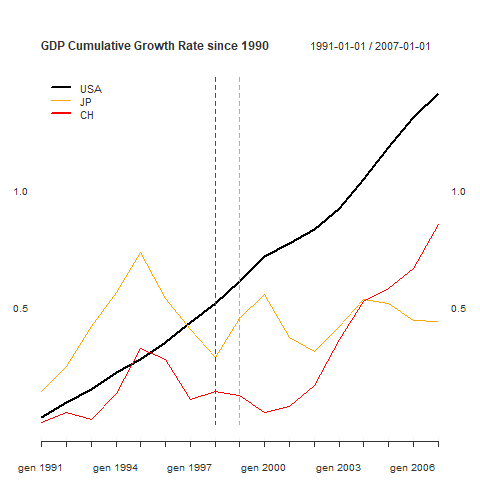
\includegraphics[width=\linewidth]{GDP.png}
    \caption{GDP cumulative growth for United States, Japan and
      Switzerland between 1990 and 2007.\\}
  \end{subfigure} \hspace{15mm} 
  \begin{subfigure}[b]{0.4\linewidth} \label{subfig:un}
    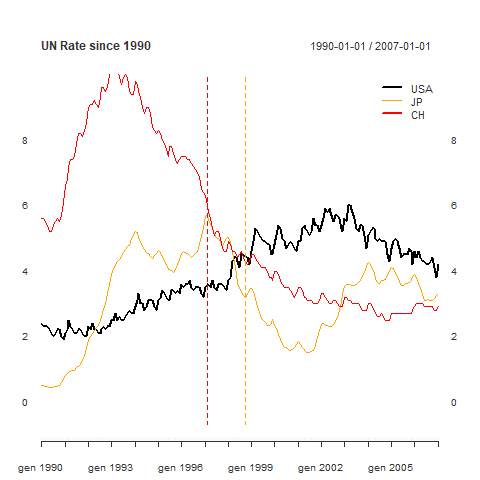
\includegraphics[width=\linewidth]{Unenployment.png}
    \caption{Percentage of working force unemployment for United States, Japan and
      Switzerland between 1990 and 2007.}
  \end{subfigure}
\vspace{2mm}\end{figure}

All of that further strengthens the generalized tree structured model
that well managed to endogenously identify such important economic
phases of the Swiss and Japanese economies once the time variable was
included in the set of variables over which to search for structural
breaks.

Important is to notice that the time splits do not influence alone the
parametric fit but stands rather in a tight relation with the other
identified threshold splits. These differ for the Swiss and the
Japanese time series. In fact, for the Japanese case the primary
regime shift depends on the American-Japanese unemployment rate
differential and the threshold value for the variable is found at the
25\% empirical quantile of the series, i.e. at -0.2\% points. This
threshold captures the period between 1994 and 1997 that is
characterized by the most rapid GDP downturn of the Japanese economy
time series as it is possible to visualize in figure \ref{fig:macro}.

For the Swiss case a second partition is instead identified depending
on the 37.5\% quantile of the logarithm of the monetary mass ratio
distribution, which very roughly represents the growth rate
differential between the USD monetary mass and the Swiss monetary mass
expressed in USD. No theoretical convincing reason could be found for
the partition and an interpretation is left to the reader and to the
economic historians.

Finally, turning to the GBP/USD generalized tree structured modeling,
three optimal threshold splits are found giving rise to four different
partitions of the data set space as visible from figure \ref{fig:UK}.
The first and foremost important difference depends on the
American-British 3-months treasury bills interest rate
differential. For the variable the threshold is selected to be the
50\% empirical quantile of the American-British interest rates
differential \textendash \ i.e. the median value corresponding roughly
to 1.8\% points. This is again an intuitive split given the importance
of the financial centers in the two countries attracting a high amount
of international capital and possibly driving FX-rates movements.

The space partitioned by the interest rates differentials is then
further refined according to the monetary mass differential and four
regimes are selected. On the left branch of the tree, the 43.75\%
quantile of the American monetary mass growth rate is selected. In the
right branch the 56.25\% quantile of the same variable is
selected. This results into four regimes: (i) one characterized by
higher than usual interest rate differentials and US-UK monetary mass
high expansion, (ii) a second characterized by higher than usual
interest rates differentials and mild US-UK monetary mass expansion,
(iii) a third consisting of a lower than usual interest rates
differential and a severe US-UK monetary mass contraction and,
finally, (iv) a fourth regime of mild US-UK monetary mass contraction
combined with lower than usual American-British interest rates
differentials.

An interesting aspect to notice in all of the mentioned cases is how
the macroeconomic variables chosen for partitioning the data set space
are the ones that proved to be co-integrated with the FX-rate series
according to the Johansen eigenvalue trace test statistic. To further
investigate such an aspect the estimated parameters for the tree
terminal nodes model fit were further inspected.

In general some key relations holds. For instance in UK case, when the
interest rates differential is below the median value, and therefore
the tree in the left branch, the foreign exchange rate differentials
are estimated to be lower \textendash \ due to the
general lower estimated coefficients \textendash \ in line with the
macroeconomic theory and the co-integration relation discussed
above. A similar results holds for the Swiss split, where the
parameters of the terminal fit in node five of figure \ref{fig:CH}
estimate ceteris paribus a lower FX-rate change in comparison to the
terminal fit in node 4 in line with the theory suggesting an
appreciating currency in a decreasing relative money supply.

Before turning to the rolling forecast analysis it is therefore
possible to claim that the obtained results for the generalized tree
structured model are in general consistent with the monetary
macroeconomic theory. Moreover, the interesting finding of parametric
estimations that fits the reversal properties of the stable long run
relation among macroeconomic fundamentals and the FX-rates documented
in the previous section are a further important result of the
generalized tree structured model that is worth to consider.

\subsubsection{Rolling Forecast Optimal Partitions}

Turning to the analysis of the rolling forecast of the generalized
tree structured model a first overview is available by looking at
table \ref{table:OptimalNumberSplits}. The table presents the number
of optimal splits according to the pruned generalized tree structured
model. As visible from the table, the number of optimal partitions
diminishes in comparison with the results of the previous section and
no time three partitions are selected to be optimal.  The root of
the result should not be searched in a poor likelihood fit of a third
partition, but rather in the reduced sample size used for the
estimation. If the previous section leveraged the entire sample for
the estimation, the rolling forecast method makes use just of three
fourth of the sample activating the 40 observations constraint at a
earlier stage and inhibiting a third space partition due to unreliable
parameter estimation.

Furthermore, it is interesting to notice the high number of times
where one partition is chosen as optimal. This is both caused by the
pruning action as well as from the small sample studied. It is namely
noted how, for instance in the British case, the final 15 optimal
splits are selected at the median value of the interest rate
differential and how the two partitions of the data set cannot be
further partitioned according to the quantiles and variables of choice
without violating the number of observation constraints.

Tables \ref{table:OptimalSplitsCH}\textendash
\ref{table:OptimalSplitsUK} further report the number each combination
of threshold variables and quantile value is chosen for the optimal
first partition in the rolling estimation and are left to the
interested reader.

Finally, table \ref{table:FullOptimalSplit} in the appendix, reports
the optimal partition tuples for the rolling generalized tree
estimation. The partitioning stays generally stable over intervals of
time. Moreover when looking at the usage rate, defined as the
percentage of time a variable enters the rolling generalized tree
estimation, it is possible to see the particular high value for the
monetary mass in the Swiss case, reaching as high as 66,7\%, and for
the Japanese case, where the monetary mass is selected to be an
optimal variable for partitioning the space in 73\% of the cases. This
confirms the importance of the monetary mass, further stressing how
the difference in the monetary mass growth differentials well signal
distinguished moments of the economies calling for a differentiated
parametric fit and differentiated macroeconomic fundamentals influence.
Nonetheless, the result seems not to be generally valid but rather
dependent of the characteristics two economies analyzed. The analysis
of the GBP/USD yield a different picture, with the monetary mass
growth rate usage scoring as low as 2\% in comparison with a usage
rate of 100\% for the interest rate difference, which interestingly
was the UK-series showing the highest statistical significance for
co-integration with the macroeconomic FX-rate series.

\subsubsection{Out-of-Sample Fit}

The final results for the out-of-sample performance fit of the rolling
generalized tree structured model estimation are presented in table
\ref{table:GTS-OLS fit}. For the table the bootstrapped superior
predictive ability p-values are omitted as being 0 for all of the
models but the generalized tree structured model. The model confidence
set procedure of Hansen (2011, \cite{HansenMCS}) rejects the Null of
equal predictive between each of the model and the generalized
structured tree performance with arbitrarily high confidence, eliminating
iteratively all of the models by keeping just the generalized tree
structured model as the best performing model.

\begin{table}[!h] % 
  \centering
    \caption[MAE \textendash \ GTS Model]{Mean Absolute Error \textendash \ Generalized Tree Structure Model}
  \begin{tabular}{llccc} % tells how you want the columns aligned.
    \toprule
    \multicolumn{5}{c}{Multivariate Models}                      \\
    \cmidrule(r){1-5}
    Lag                           &   Model                                     &Switzerland  & Japan     & United Kingdom\\
    \midrule
    \multirow{4}{*}{MAE 1}        & \multicolumn{1}{l}{Random Walk}             &   0.0193  & 0.0168  & 0.0162 \\  
                                  & \multicolumn{1}{l}{VAR}                     &   0.0183  & 0.0186  & 0.0160 \\ 
                                  & \multicolumn{1}{l}{VECM}                    &   0.0176  & 0.0174  & 0.0153 \\
                                  & \multicolumn{1}{l}{GTS-OLS}                 &   0.0082  & 0.0084  & 0.0101 \\    
    \\
    \multirow{4}{*}{MAE 3}        & \multicolumn{1}{l}{Random Walk}             &   0.0390  & 0.0330  & 0.0291 \\ 
                                  & \multicolumn{1}{l}{VAR}                     &   0.0394  & 0.0333  & 0.0292 \\
                                  & \multicolumn{1}{l}{VECM}                    &   0.0376  & 0.0328  & 0.0320 \\
                                  & \multicolumn{1}{l}{GTS-OLS}                 &   0.0089  & 0.0081  & 0.0096 \\
    \\
    \multirow{4}{*}{MAE 6}        & \multicolumn{1}{l}{Random Walk}             &   0.0580  & 0.0495  & 0.0439 \\
                                  & \multicolumn{1}{l}{VAR}                     &   0.0578  & 0.0488  & 0.0418 \\
                                  & \multicolumn{1}{l}{VECM}                    &   0.0580  & 0.0483  & 0.0434 \\
                                  & \multicolumn{1}{l}{GTS-OLS}                 &   0.0075  & 0.0080  & 0.0099 \\    
     \\
    \multirow{4}{*}{MAE 12}       & \multicolumn{1}{l}{Random Walk}             &   0.0964  & 0.0584  & 0.0753 \\
                                  & \multicolumn{1}{l}{VAR}                     &   0.0974  & 0.0603  & 0.0763 \\
                                  & \multicolumn{1}{l}{VECM}                    &   0.0881  & 0.0542  & 0.0731 \\
                                  & \multicolumn{1}{l}{GTS-OLS}                 &   0.0078  & 0.0088  & 0.0095 \\    
    \bottomrule
  \end{tabular}
  \label{table:GTS-OLS fit}
  \vspace{1em}  
\end{table}

Interestingly is to notice the performance of the generalized tree
structured model out-of-sample. The model consistently and
significantly reduce the out of sample error independently on whether
the latter is measured in terms MAE or RSME terms. Moreover, it
manages to increase the mean directional accuracy to levels ranging
between 80\%-90\%, a 30\%-40\% increase.

When looking at table \ref{table:GTS-OLS fit}, the results are
clear. The generalized tree structured model menages to increase the
out of sample fit by around 50\% on the one month lag out-of-sample
estimation. Moreover, the performance of the model seems not to
constantly deteriorate with an increasing out-of-sample estimation lag
but stays rather constant, therefore strongly improving the
out-of-sample-fit at higher lags.


\subsubsection{Multivariate model fit}

Given the strong performance of the univariate parametric fit in the
generalized tree structured model a multivariate generalized tree
structured model estimation was tried with a vector error correction
model and a vector auto-regressive model fit in the final nodes of the
tree.

Given the high number of parameters in such multivariate models the
criteria for further partitioning the tree was adjusted to 80+
observations. The generalized tree structured model could not go
beyond one threshold variable and two partitions for the model due to
the higher stopping criteria. Moreover, the out-of-sample performance
deteriorated sensibly in comparison to the not partitioned
multivariate models suggesting over fitting issues. The conclusion was
further supported by the further worsen of performance of models with
70 observation stopping criteria threshold allowing to select
threshold splits further in the tails of the empirical variable
distribution.

Due to restricted sample size it is therefore not possible to draw
sensible conclusions for the generalized tree structured model with
multivariate model end-node parametric fit and the paper abstains
therefore for conclusive remarks about the performance of the models
leaving it as an interesting opportunity for research for the years to
come.

\section{Criticalities}

The results outlined presented in the study underline the strong
evidence for a long run stable relation among macroeconomic
fundamentals and FX-rates.

The promising results from the generalized tree structured model
further suggest the importance of capturing the stochastic process of
FX-rates by incorporating different regimes based on the underlying
macroeconomic situation. This result, together with the estimation of
parameters in line with the reversal property that guarantees the long
term stable relation among macroeconomic fundamentals and FX-rates
might suggest how the adjustment process to the stable long run
equilibrium is rather unstable through time and requires therefore a
sluggish adjustment process as the one of alternating regime rather
than a gradual, periodic, adjustment as the one modeled by the
vector error correction model.

Despite, the above achievements some structural flows remain in the
analysis. Starting, with a theoretical notice, it should be mentioned
how all of the four currencies analyzed are considered to be safe haven
currencies in the broad academic literature. This, implies that
important movements for the series might be affected by important
political events as documented by Ranaldo and S{\"o}derlind (2010,
\cite{RanaldoSoderlind}) rather then by macroeconomic fundamental
movements leading to a worsen performance of the structural monetary
fit. Interesting would be in this sense to analyze the results for
other less liquid FX-rates series and observe whether the results are
in line with the one presented in the analysis as well as in the
benchmark papers.

Moreover, some general issues remain with the macroeconomic proxies
used in the analysis. Figure \ref{fig:macro} shows how the
unemployment rate and the gross domestic product growth are generally
negatively correlated supporting the validity of proxy of choice,
nonetheless, the possibility of further supporting the results by
leveraging a linear interpolation of the GDP level or the crude oil
consumption level subsist. 

Finally, albeit the generalized tree structured model well managed to
significantly outperform a random walk model, it should be further
stressed the different information set leveraged by the model
suggesting caution in claiming a claiming the superiority of the
generalized tree structured model for modeling FX-rates
out-of-sample.




